% Latex课程报告模板
 
\documentclass{article}

\usepackage[UTF8]{ctex}
\usepackage{geometry}
\geometry{paper=a4paper}
\usepackage{graphicx}
\usepackage{gbt7714}

\begin{document}

\thispagestyle{empty}
\begin{figure}[h]
    \centering
    
\includegraphics[width=0.8\textwidth]{./城院logo1.png}
    % \caption{}
\end{figure}
% \vspace*{12em}
\begin{center}
{\Huge 自然辩证法期末作业}\\
\end{center}
\begin{figure}[h]
    \centering
    
\includegraphics[width=0.25\textwidth]{./城院logo2.png}
    % \caption{}
\end{figure}
\vspace{10em}
\begin{center}
{\Large  % 这里的字号也可以用别的方式修改
\makebox[4em][s]{题目}:\hspace{1em}\underline{\makebox[18em][c]{马克思主义自然观与科学技术观之感想}}\\
\makebox[4em][s]{姓名}:\hspace{1em}\underline{\makebox[18em][c]{周卓}}\\
\makebox[4em][s]{学号}:\hspace{1em}\underline{\makebox[18em][c]{2240201012}}\\
\makebox[4em][s]{专业班级}:\hspace{1em}\underline{\makebox[18em][c]{电子信息2402}}\\
\makebox[4em][s]{学院}:\hspace{1em}\underline{\makebox[18em][c]{信息与电气工程学院}}\\
\makebox[4em][s]{任课老师}:\hspace{1em}\underline{\makebox[18em][c]{胡小波、应腾、张义修}}\\
}
\end{center}






\title{马克思主义自然观与科学技术观之感想}
\author{周卓 2240201012}
\date{\today}
\maketitle
\thispagestyle{empty}

\begin{abstract}
    本文首先介
    
    \textbf{关键字:} 预后模型,机器学习,智能诊断
\end{abstract}

\newpage
\pagenumbering{roman}
\tableofcontents
\newpage
\pagenumbering{arabic}

\section{预后模型概念}
    \subsection{基本概念}
    临床预测概率\cite{chen2020overview}.

    步骤\ref{fig:a}.
    \begin{figure}[h]
        \centering
        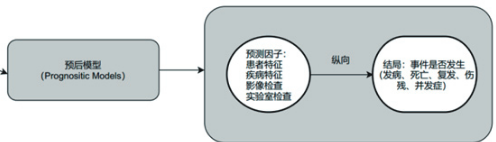
\includegraphics[width=0.5\textwidth]{2fig/a.png}
        \caption{预后模型概念}
        \label{fig:a}
    \end{figure}
    
\section{预后建模方法}
    \subsection{确立研究问题}
    
    
    \subsection{选择数据来源}

    \subsection{筛选预测变量}
   
    \subsection{处理预测变量}
    

    \subsection{拟合预测模型}
    
    \subsection{评估预测模型}
    
    
\section{机器学习在医疗领域中的应用}

    \subsection{疾病预测}
        高达84\%\cite{伍亚舟2022人工智能在临床领域的研究进展及前景展望}. 
    \begin{figure}[h]
        \centering
        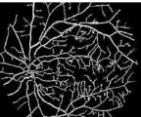
\includegraphics[width=0.5\textwidth]{2fig/b.png}
        \caption{识别血管网}
        \label{fig:b}
    \end{figure}
        
    \subsection{疾病辅助诊断}
    

\section{预后建模的挑战}
    \subsection{数据很难收集}

    \subsection{$x$数据不完备,即数据删失}

    \subsection{$\hat{y} $信息不完备,$\hat{y} $多事件且有互斥}

    \subsection{深度预后模型的可解释性}

    \subsection{数据分布偏差, 专家知识如何介入}
\newpage


\bibliographystyle{gbt7714-numerical}
\bibliography{2}



\end{document}